% -*- latex -*-
%%%%%%%%%%%%%%%%%%%%%%%%%%%%%%%%%%%%%%%%%%%%%%%%%%%%%%%%%%%%%%%%
%%%%%%%%%%%%%%%%%%%%%%%%%%%%%%%%%%%%%%%%%%%%%%%%%%%%%%%%%%%%%%%%
%%%%
%%%% This text file is part of the source of 
%%%% `Parallel Programming in MPI and OpenMP'
%%%% by Victor Eijkhout, copyright 2012-7
%%%%
%%%% mpi-derived.tex : derived datatypes
%%%%
%%%%%%%%%%%%%%%%%%%%%%%%%%%%%%%%%%%%%%%%%%%%%%%%%%%%%%%%%%%%%%%%
%%%%%%%%%%%%%%%%%%%%%%%%%%%%%%%%%%%%%%%%%%%%%%%%%%%%%%%%%%%%%%%%

\Level 0 {Derived datatypes}
\label{sec:derived-types}
\index{datatype!derived|(}

MPI allows you to create your own data types, somewhat (but not completely\ldots)
analogous to defining
structures in a programming language. MPI data types are mostly of use
if you want to send multiple items in one message.

There are two problems with using only elementary datatypes
as you have seen so far.
\begin{itemize}
\item MPI communication routines can only send multiples of a
  single data type: it is not possible to send items of different
  types, even if they are contiguous in memory. It would be possible
  to use the \n{MPI_BYTE} data type, but this is not advisable.
\item It is also ordinarily not possible to send items of one type if they are
  not contiguous in memory. You could of course send a contiguous memory area
  that contains the items you want to send, but that is wasteful of
  bandwidth.
\end{itemize}
With MPI data types you can solve these problems in several ways.
\begin{itemize}
\item You can create a new \indextermbus{contiguous}{data type}
  consisting of an array of elements of another data type. There is no
  essential difference between sending one element of such a type
  and multiple elements of the
  component type.
\item You can create a \indextermbus{vector}{data type} consisting of
  regularly spaced blocks of elements of a component type. This is a first
  solution to the problem of sending non-contiguous data.
\item For not regularly spaced data, there is the
  \indextermbus{indexed}{data type}, where you specify an array of
  index locations for blocks of elements of a component type.
  The blocks can each be of a different size.
\item The \indextermbus{struct}{data type} can accomodate multiple
  data types.
\end{itemize}
And you can combine these mechanisms to get irregularly spaced
heterogeneous data, et cetera.

\Level 1 {Basic calls}
\label{sec:data-commit}

The typical sequence of calls for creating a new datatype is as follows:
\begin{verbatim}
MPI_Datatype newtype;
MPI_Type_<sometype>( < oldtype specifications >, &newtype );
MPI_Type_commit( &newtype );
/* code that uses your new type */
MPI_Type_free( &newtype );
\end{verbatim}

\Level 2 {Datatype objects}

MPI derived data types are stored in variables of type
\indexmpishow{MPI_Datatype}.
%
\mpiRoutineRef{MPI_Datatype}

\Level 2 {Create calls}

The \indexmpishow{MPI_Datatype} varriable gets its value by a call to
one of the following routines:
\begin{itemize}
\item \indexmpishow{MPI_Type_contiguous} for contiguous blocks of
  data; section~\ref{sec:data:contiguous};
\item \indexmpishow{MPI_Type_vector} for regularly strided data;
  section~\ref{sec:data:vector};
\item \indexmpishow{MPI_Type_create_subarray} for subsets out higher
  dimensional block; section~\ref{sec:type_subarray};
\item \indexmpishow{MPI_Type_struct} for heterogeneous irregular data;
  section~\ref{sec:data:struct};
\item \indexmpishow{MPI_Type_indexed} and
  \indexmpishow{MPI_Type_hindexed} for irregularly strided data;
  section~\ref{sec:data:indexed}.
\end{itemize}
These calls take an existing type, whether elementary or also derived,
and produce a new type.

\Level 2 {Commit and free}

It is necessary to call \indexmpishow{MPI_Type_commit} on a new data
type, which makes MPI do the indexing calculations for the data type.
%
\mpiRoutineRef{MPI_Type_commit}

When you no longer
need the data type, you call \indexmpishow{MPI_Type_free}.
\begin{verbatim}
int MPI_Type_free (MPI_datatype *datatype)
\end{verbatim}
\begin{itemize}
\item The definition of the datatype identifier will be changed to
  \indexmpishow{MPI_DATATYPE_NULL}.
\item Any communication using this data type, that was already
  started, will be completed succesfully.
\item Datatypes that are defined in terms of this data type will still
  be usable.
\end{itemize}

\Level 1 {Contiguous type}
\label{sec:data:contiguous}

The simplest derived type is the `contiguous' type,
constructed with \indexmpishow{MPI_Type_contiguous}.
%
\mpiRoutineRef{MPI_Type_contiguous}
%
A~contigous type describes an array of items
of an elementary or earlier defined type. There is no difference between sending
one item of a contiguous type and multiple items of the constituent type.
\begin{figure}[ht]
  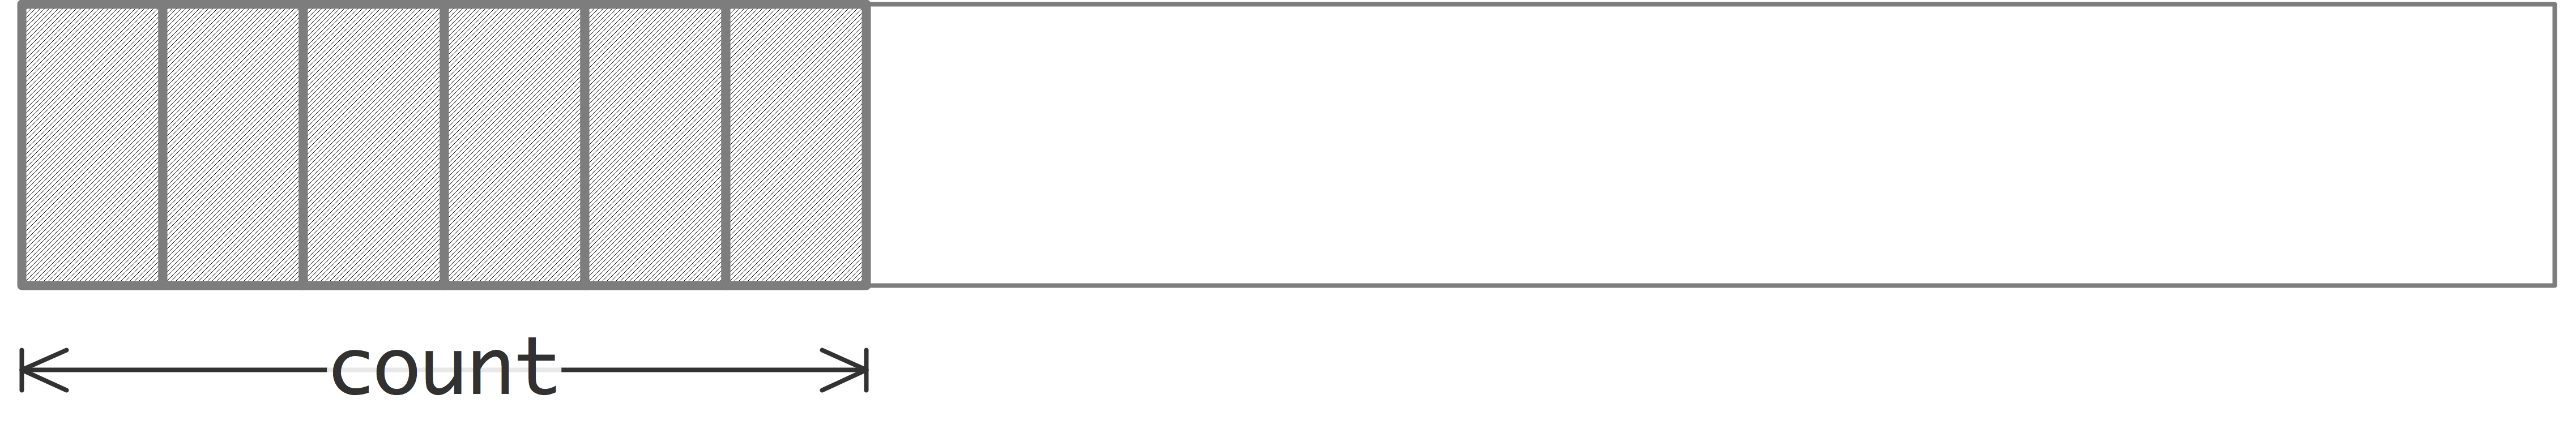
\includegraphics[scale=.08]{data-contiguous}
  \caption{A contiguous datatype is built up out of elements of a constituent type}
  \label{fig:data-contiguous}
\end{figure}
This is illustrated in figure~\ref{fig:data-contiguous}.

\verbatimsnippet{contiguous}

\Level 1 {Vector type}
\label{sec:data:vector}

The simplest non-contiguous datatype is the `vector' type, constructed with
\indexmpishow{MPI_Type_vector}.
%
\mpiRoutineRef{MPI_Type_vector}
%
A~vector type describes a series of blocks, all 
of equal size, spaced with a constant stride.
\begin{figure}[ht]
  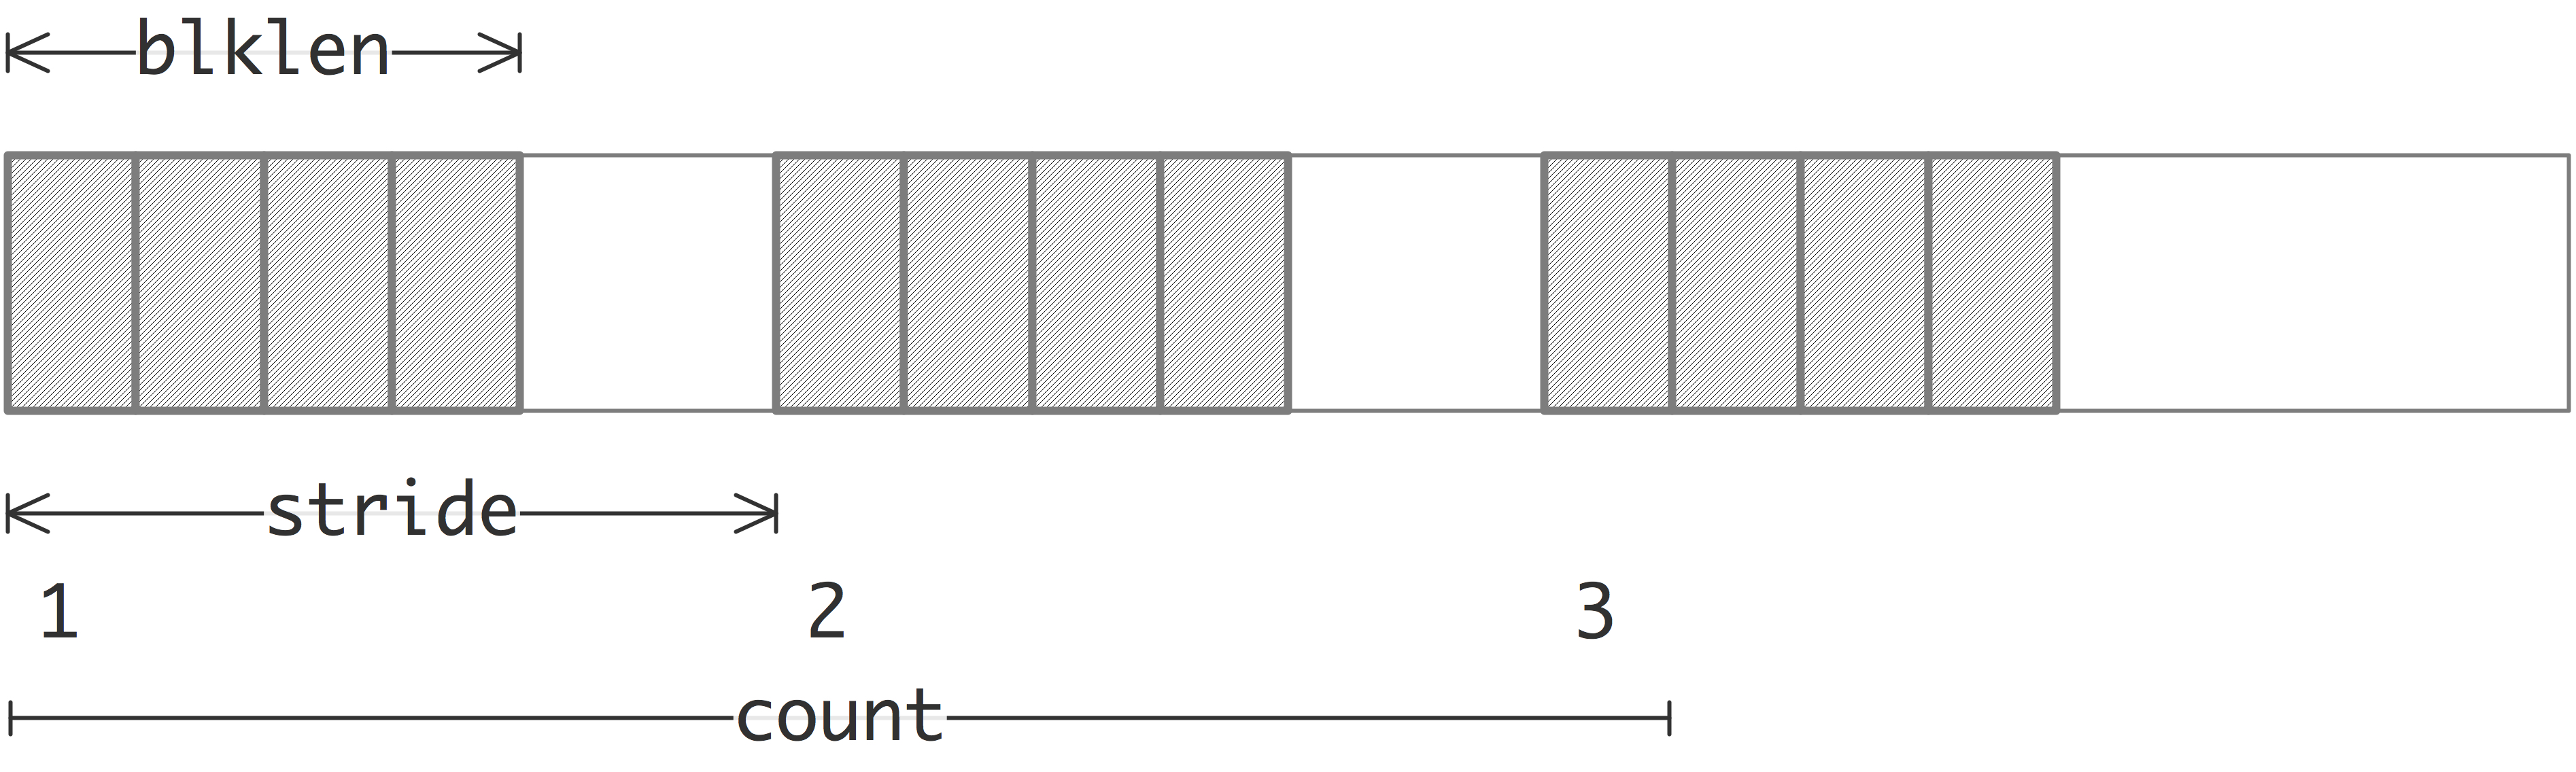
\includegraphics[scale=.12]{data-vector}
  \caption{A vector datatype is built up out of strided blocks of elements of a constituent type}
  \label{fig:data-vector}
\end{figure}
This is illustrated in figure~\ref{fig:data-vector}.

The vector datatype gives the first non-trivial illustration that
datatypes can be \emph{different on the sender and
  receiver}\index{datatype!different on sender and receiver}. If the
sender sends \n{b}~blocks of length~\n{l} each, the receiver can
%
\begin{figure}
  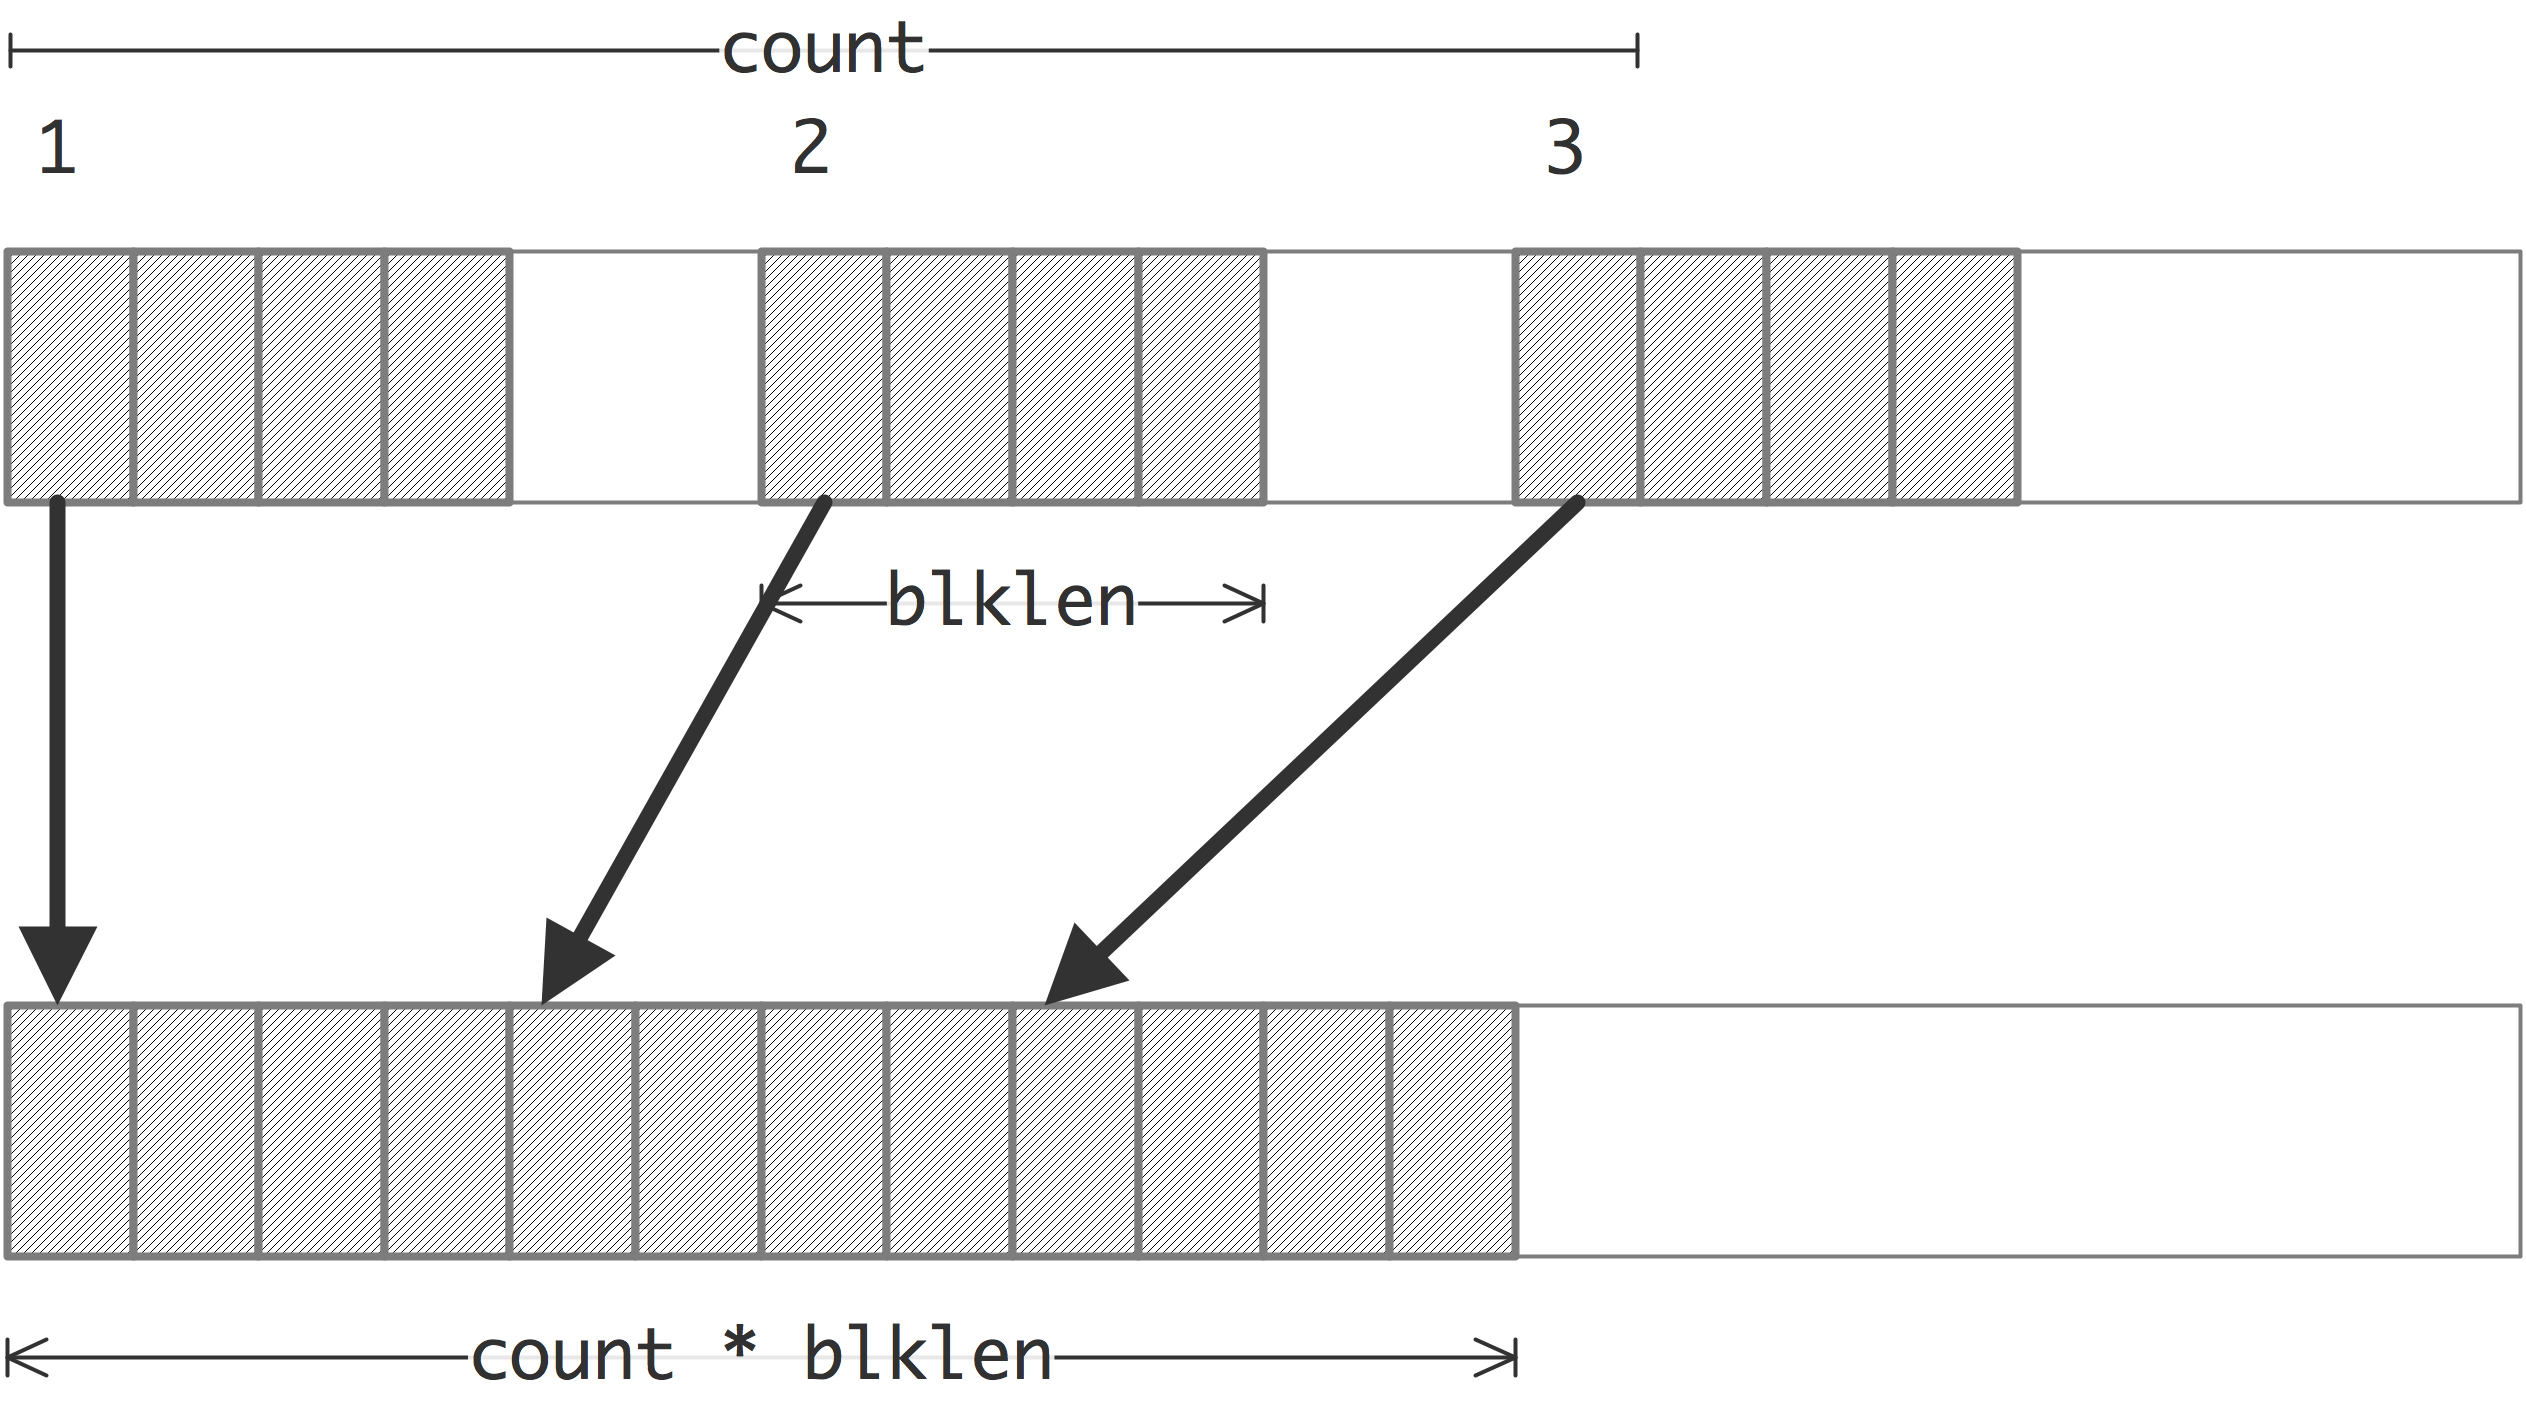
\includegraphics[scale=.12]{data-vector-to-contiguous}
  \caption{Sending a vector datatype and receiving it as elementary or
    contiguous}
  \label{fig:data-vector-to-contiguous}
\end{figure}
%
receive them as \n{bl} contiguous elements, either as a contiguous
datatype, or as a contiguous buffer of an elementary type; see
figure~\ref{fig:data-vector-to-contiguous}. In this case, the receiver
has no knowledge of the stride of the datatype on the sender.

In this example a vector type is created only on the sender, in order to send
a strided subset of an array; the receiver receives the data as a contiguous block.
\verbatimsnippet{vector}

As an example of this datatype, consider the example of transposing
a matrix, for instance to convert between
C and Fortran arrays (see section~\HPSCref{sec:CFarrays}). Suppose that 
a processor has a matrix stored in~C, row-major, layout, and it needs
to send a column to another processor. If the matrix is declared as
\begin{verbatim}
  int M,N; double mat[M][N]
\end{verbatim}
then a column has $M$ blocks of one element, spaced $N$~locations apart.
In other words:
\begin{verbatim}
MPI_Datatype MPI_column;
MPI_Type_vector( 
    /* count= */ M, /* blocklength= */ 1, /* stride= */ N,
    MPI_DOUBLE, &MPI_column );
\end{verbatim}
Sending the first column is easy:
\begin{verbatim}
MPI_Send( mat, 1,MPI_column, ... );
\end{verbatim}
The second column is just a little trickier: you now need to pick out 
elements with the same stride, but starting at \n{A[0][1]}.
\begin{verbatim}
MPI_Send( &(mat[0][1]), 1,MPI_column, ... );
\end{verbatim}
You can make this marginally more efficient (and harder to read)
by replacing the index expression by \n{mat+1}.

\begin{exercise}
  Suppose you have a matrix of size $4N\times 4N$, and you want to
  send the elements \n{A[4*i][4*j]} with $i,j=0,\ldots,N-1$. How would
  you send these elements with a single transfer?
\end{exercise}

\begin{exercise}
  \label{ex:col-to-row}
  Allocate a matrix on processor zero, using Fortran column-major storage.
  Using $P$ sendrecv calls, distribute the rows of this matrix among the
  processors.
\end{exercise}

\begin{exercise}
  \label{ex:stridesend}
  Let processor~0 have an array~$x$ of length $10P$, where $P$~is the number of processors.
  Elements $0,P,2P,\ldots,9P$ should go to processor zero, $1,P+1,2P+1,\ldots$ to processor~1,
  et cetera. Code this as a sequence of send/recv calls, using a vector datatype
  for the send, and a contiguous buffer for the receive.

  For simplicity, skip the send to/from zero. What is the most elegant
  solution if you want to include that case?

  For testing, define the array as $x[i]=i$.
\end{exercise}

\begin{exercise}
  Write code to compare the time it takes to send a strided subset
  from an array: copy the elements by hand to a smaller buffer, or use
  a vector data type. What do you find?
\end{exercise}

\Level 2 {Subarrays as vector data}

Figure~\ref{fig:blasmatrix} indicates one source of irregular
data:
%
\begin{figure}[ht]
  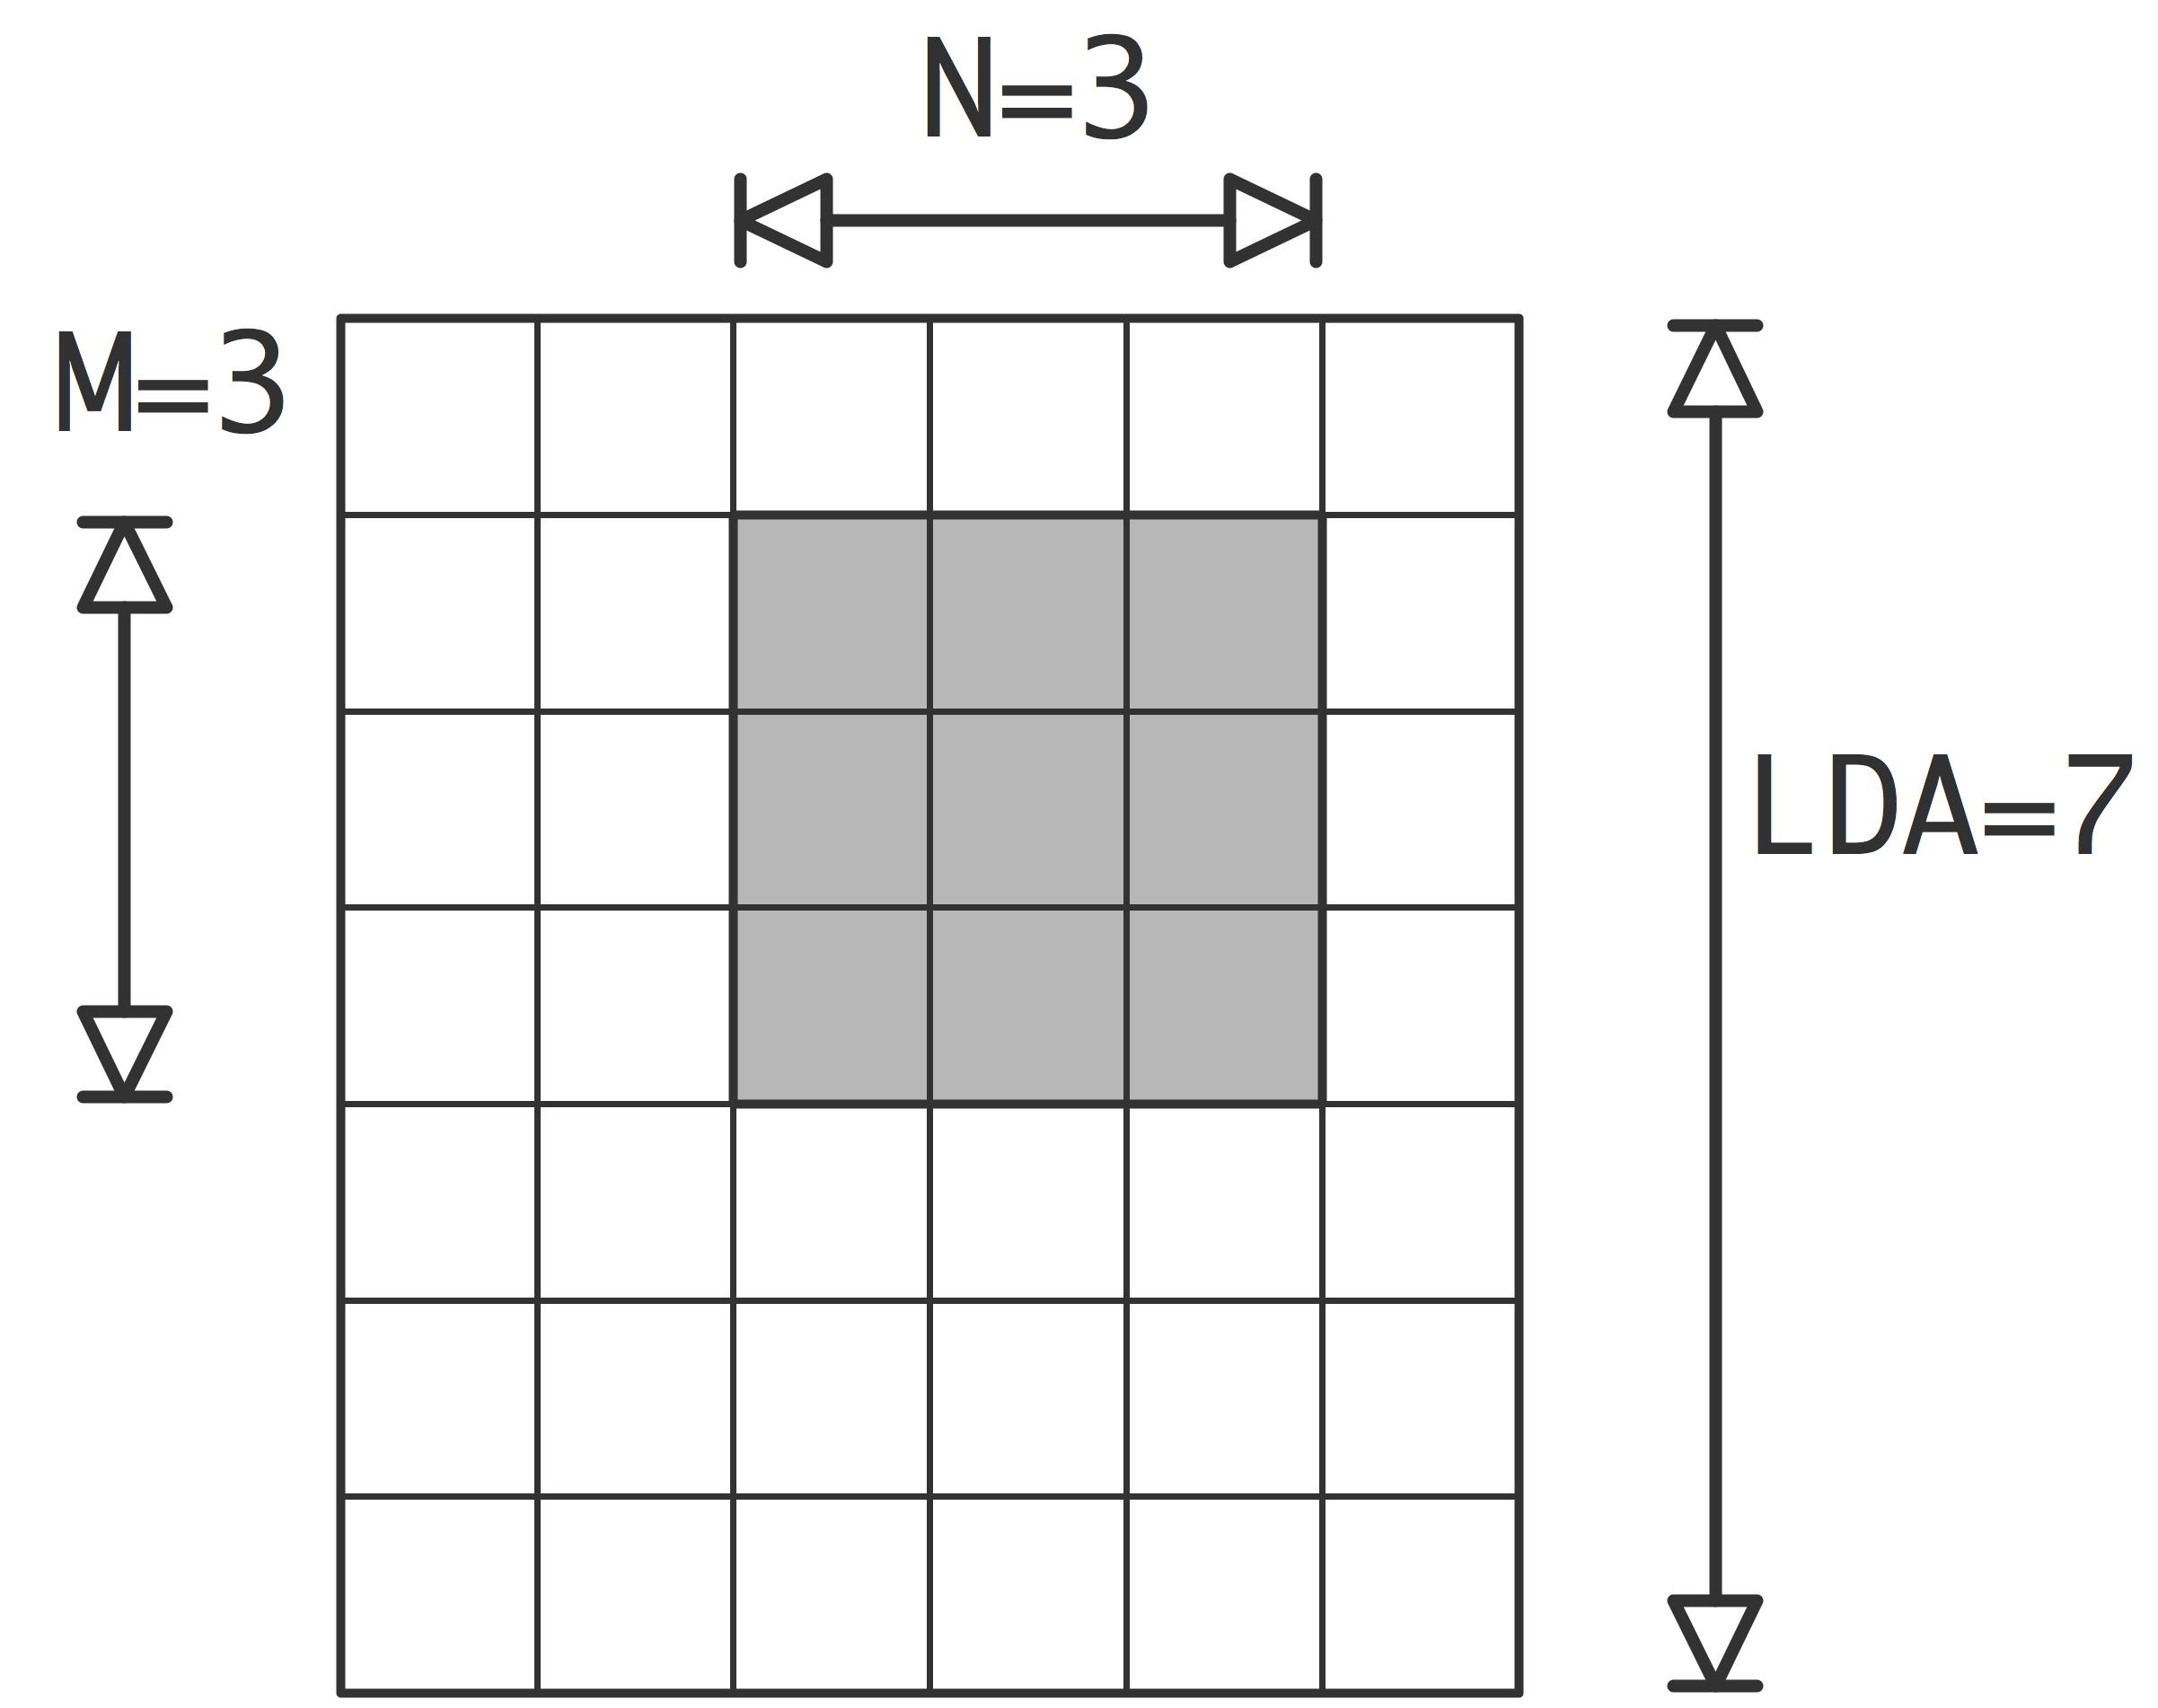
\includegraphics[scale=.1]{blasmatrix}
  \caption{Memory layout of a row and column of a matrix in column-major storage}
  \label{fig:blasmatrix}
\end{figure}
%
with a matrix on \indexterm{column-major storage}, a column is
stored in contiguous memory. However, a row of such a matrix
is not contiguous; its elements being separated by a \indexterm{stride}
equal to the column length.

\begin{exercise}
  \label{ex:submatrix}
  How would you describe the memory layout of a submatrix,
  if the whole matrix has size $M\times N$ and the submatrix $m\times n$?
\end{exercise}

\Level 2 {Subarray type}
\label{sec:type_subarray}

The vector datatype can be used for blocks in an array of dimension
more than~2 by using it recursively. However, this gets
tedious. Instead, there is an explicit subarray type
%
\mpiRoutineRef{MPI_Type_create_subarray}
%
This describes the dimensionality and extent of the array, and
the starting point (the `upper left corner') and extent of the
subarray.
The possibilities for the \n{order} parameter are
\indexmpidef{MPI_ORDER_C} and \indexmpidef{MPI_ORDER_FORTRAN}.

\begin{exercise}
  \label{ex:cubegather}

  Assume that your number of processors is $P=Q^3$, and that each
  process has an array of identical size. Use
  \n{MPI_Type_create_subarray} to gather all data onto a root process.
  Use a sequence of send and receive calls;
  \indexmpishow{MPI_Gather} does not work here.

\begin{tacc}
This is one of the rare cases where you should use \n{ibrun -np 27}
and such: normally you use \n{ibrun} without process count argument.
\end{tacc}

\end{exercise}

\Level 1 {Indexed type}
\label{sec:data:indexed}

The indexed datatype, constructed with \indexmpishow{MPI_Type_indexed}
can send arbitrarily located elements from an array of a single datatype.
You need to supply an array of index locations, plus an array of blocklengths
with a separate blocklength for each index. The total number of elements sent
is the sum of the blocklengths.
%
\mpiRoutineRef{MPI_Type_indexed}
%

\begin{figure}[ht]
  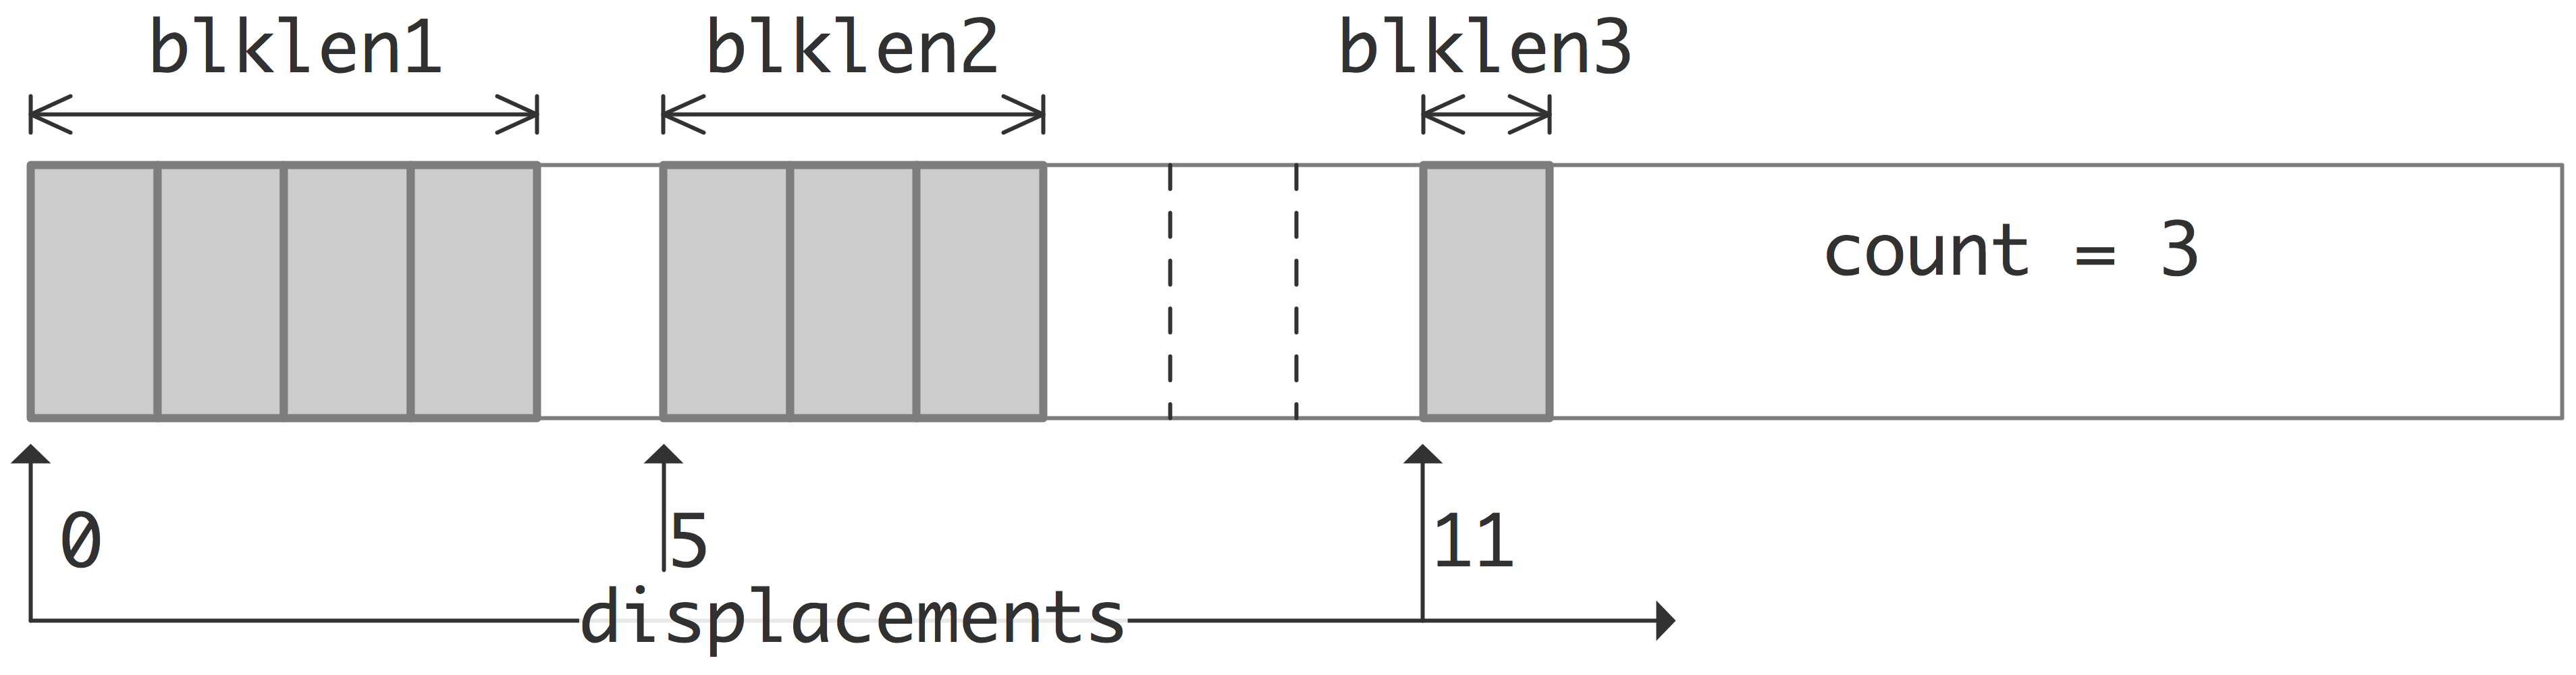
\includegraphics[scale=.11]{data-indexed}
  \caption{The elements of an MPI Indexed datatype}
  \label{fig:data-indexed}
\end{figure}

The following example picks items that are on prime number-indexed
locations.
\verbatimsnippet{indexed}

You can also \indexmpishow{MPI_Type_create_hindexed} which describes blocks
of a single old type, but with indix locations in bytes, rather than
in multiples of the old type.
\begin{verbatim}
int MPI_Type_create_hindexed
 (int count, int blocklens[], MPI_Aint indices[],
  MPI_Datatype old_type,MPI_Datatype *newtype)
\end{verbatim}
You can use this to pick all occurrences of a single component out of
an array of structures. However, you need to be very careful with the
index calculation. Use pointer arithmetic, as in the example in
section~\ref{ref:data:struct}.  Another use of this function is in
sending an \n{stl<vector>}\index{C++!standard library!vector}, that
is, a vector object from the \indextermbus{C++}{standard library}, if
the component type is a pointer. No further explanation here.

\Level 1 {Struct type}
\label{sec:data:struct}

The structure type, created with \indexmpishow{MPI_Type_create_struct},
can contain multiple data types.
%
\begin{figure}[ht]
  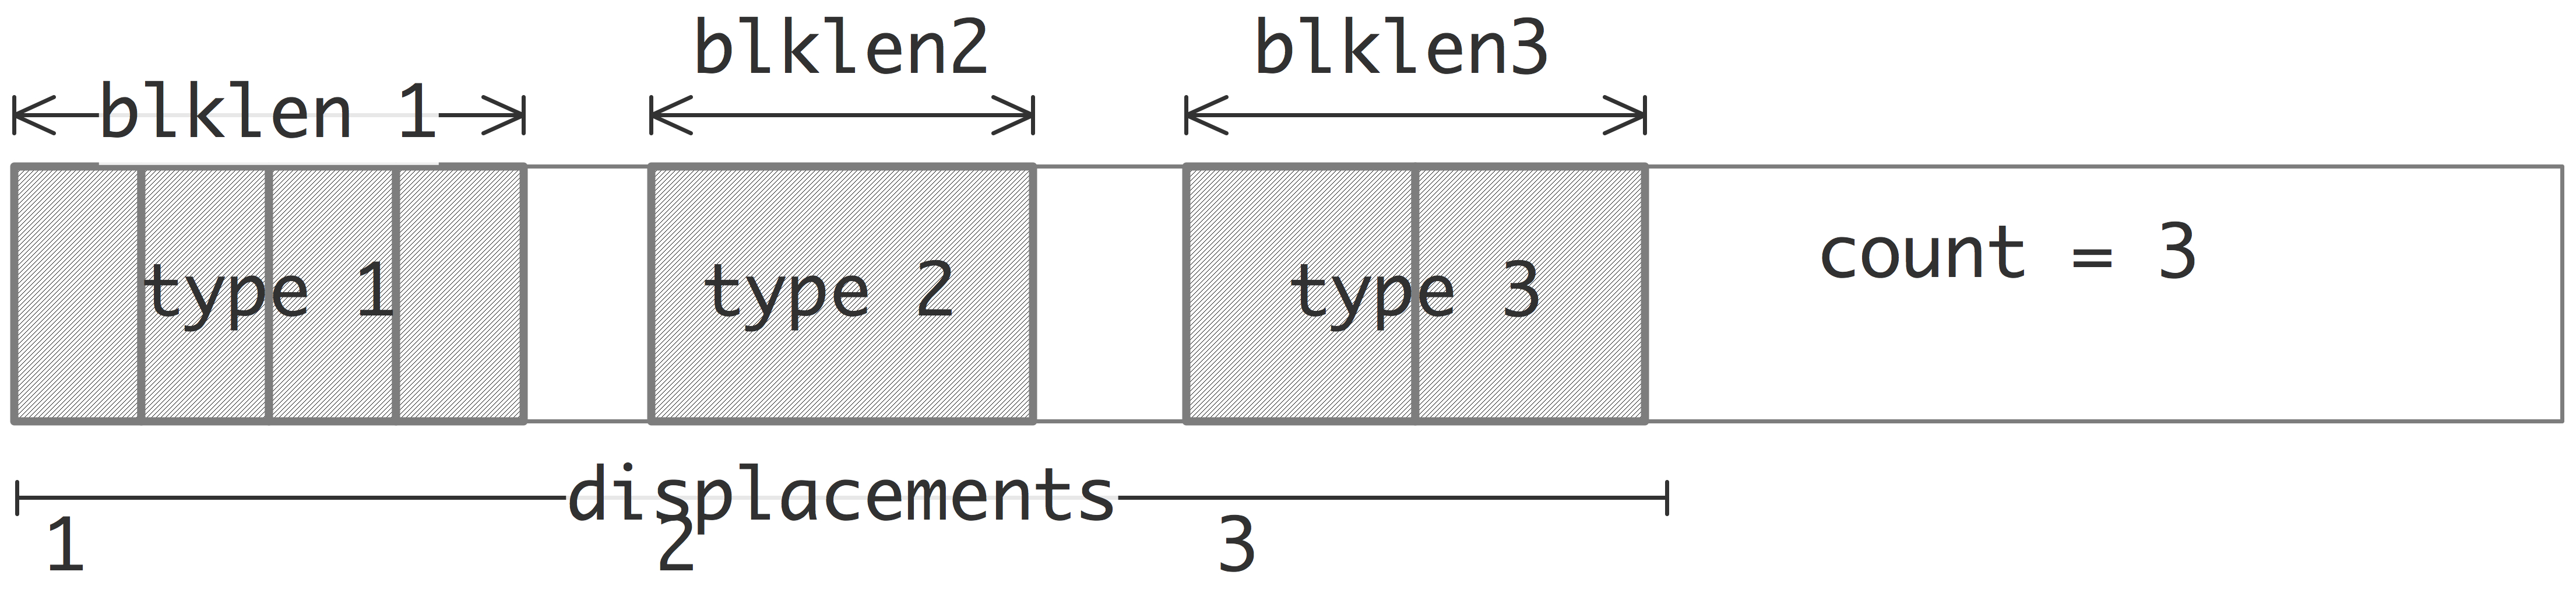
\includegraphics[scale=.11]{data-struct}
  \caption{The elements of an MPI Struct datatype}
  \label{fig:data-struct}
\end{figure}
%
The specification contains a `count' parameter that specifies how many blocks
there are in a single structure. For instance,
\begin{verbatim}
struct {
 int i;
 float x,y;
} point;
\end{verbatim}
has two blocks, one of a single integer, and one of two floats.
This is illustrated in figure~\ref{fig:data-struct}.

\begin{verbatim}
int MPI_Type_create_struct(
  int count, int blocklengths[], MPI_Aint displacements[],
  MPI_Datatype types[], MPI_Datatype *newtype);
\end{verbatim}

\begin{description}
\item[\texttt{count}] The number of blocks in this
  datatype. The \n{blocklengths}, \n{displacements}, \n{types}
  arguments have to be at least of this length.
\item[\texttt{blocklengths}] array containing the lengths of the blocks of each datatype.
\item[\texttt{displacements}] array describing the relative location
  of the blocks of each datatype.
\item[\texttt{types}] array containing the datatypes; each block in
  the new type is of a single datatype; there can be multiple
  blocks consisting of the same type.
\end{description}
In this example, unlike the previous ones, both sender and receiver
create the structure type. With structures it is no longer possible to
send as a derived type and receive as a array of a simple type.
(It would be possible to send as one structure type and receive as another, 
as long as they have the same \indextermbus{datatype}{signature}.)
%
\verbatimsnippet{structure}
%
Note the \n{displacement} calculations in this example,
which involve some not so elegant pointer arithmetic.
It would have been incorrect to write
\begin{verbatim}
displacement[0] = 0;
displacement[1] = displacement[0] + sizeof(char);
\end{verbatim}
since you do not know the way the \indexterm{compiler} lays out the
structure in memory\footnote{Homework question: what does the language
  standard say about this?}.

If you want to send more than one structure, you have to worry more
about padding in the structure. You can solve this by adding an extra
type \indexmpishow{MPI_UB} for the `upper bound' on the structure:
\begin{verbatim}
displacements[3] = sizeof(myobject); types[3] = MPI_UB;
MPI_Type_create_struct(struclen+1,.....);
\end{verbatim}

The structure type is very similar in functionality to \indexmpishow{MPI_Type_hindexed},
which uses byte-based indexing. The structure-based type is probably cleaner
in use.

\Level 1 {Examples}

\mpiRoutineRef{MPI_Type_contiguous}

We send a contiguous data type of double and receive it as an array of
separate doubles; we use \indexmpishow{MPI_Get_count} to ensure that
we got the right amount of data.
%
\verbatimsnippet{contiguous}
%
\verbatimsnippet{contiguous-f}

\mpiexample{MPI_Type_indexed}

We send an indexed data type and receive as separate integers.
%
\verbatimsnippet{indexed}
%
\verbatimsnippet{indexed-f}
%
\verbatimsnippet{indexp}

\mpiexample{MPI_Type_struct}

A struct data type can consist of different elementary datatypes, so
in addition to the displacements and blocklengths we now have an array
of MPI datatypes. Also note how the displacement computation is done
in bytes.
%
\verbatimsnippet{structure}

\mpiexample{MPI_Type_vector}

Send a strided data object with \n{Type_vector} and receive it as
individual doubles. Use \indexmpishow{MPI_Get_count} to inspect the
\n{MPI_Status} object.
%
\verbatimsnippet{vector}
%
\verbatimsnippet{vector-f}
%
\verbatimsnippet{vectorp}

\Level 1 {Type size}

The space that MPI takes for a structure type can be queried in a
variety of ways. First of all \indexmpishow{MPI_Type_size} counts the
\emph{datatype size}\index{MPI!datatype!size} as the 
number of bytes occupied by the data in a type. That means that in an
\emph{MPI vector datatype}\index{MPI!datatype!vector} it does not
count the gaps.
%
\verbatimsnippet{vectortypesize}
%
\mpiRoutineRef{MPI_Type_size}

On the other hand, the \emph{datatype
  extent}\index{MPI!datatype!extent} is strictly the distance from the
first to the last data item of the type, that is, with counting the
gaps in the type.
%
\verbatimsnippet{vectortypeextent}
%
\mpiRoutineRef{MPI_Type_get_extent}
%
(There is a deprecated function \indexmpishow{MPI_Type_extent} with the same
functionality.)

The \emph{subarray datatype}\index{MPI!datatype!subarray} need not
start at the first element of the buffer, so the extent is an
overstatement of how much data is involved. The routine
\indexmpishow{MPI_Type_get_true_extent} returns the lower bound,
indicating where the data starts, and the extent from that point.
%
\mpiRoutineRef{MPI_Type_get_true_extent}

\begin{comment}
  Suppose we implement gather (see also Section Gather ) as a spanning
  tree implemented on top of point-to-point routines. Since the receive
  buffer is only valid on the root process, one will need to allocate
  some temporary space for receiving data on intermediate
  nodes. However, the datatype extent cannot be used as an estimate of
  the amount of space that needs to be allocated, if the user has
  modified the extent, for example by using MPI_TYPE_CREATE_RESIZED. The
  functions MPI_TYPE_GET_TRUE_EXTENT and MPI_TYPE_GET_TRUE_EXTENT_X are
  provided which return the true extent of the datatype.
\end{comment}

\verbatimsnippet{trueextent}
